\documentclass[10pt, conference, compsocconf]{IEEEtran}

% *** GRAPHICS RELATED PACKAGES ***
%
\ifCLASSINFOpdf
  % \usepackage[pdftex]{graphicx}
  % declare the path(s) where your graphic files are
  % \graphicspath{{../pdf/}{../jpeg/}}
  % and their extensions so you won't have to specify these with
  % every instance of \includegraphics
  % \DeclareGraphicsExtensions{.pdf,.jpeg,.png}
\else
  % or other class option (dvipsone, dvipdf, if not using dvips). graphicx
  % will default to the driver specified in the system graphics.cfg if no
  % driver is specified.
  % \usepackage[dvips]{graphicx}
  % declare the path(s) where your graphic files are
  % \graphicspath{{../eps/}}
  % and their extensions so you won't have to specify these with
  % every instance of \includegraphics
  % \DeclareGraphicsExtensions{.eps}
\fi

\bibliographystyle{IEEEtran}

\usepackage{graphicx}
\usepackage{subcaption}
\usepackage{booktabs}
\usepackage{caption}
\usepackage[table,xcdraw]{xcolor}
\usepackage{flafter}
\usepackage{refstyle}
\usepackage{amsmath}
\usepackage{amsthm}

\graphicspath{ {images/} }

%\usepackage{subfiles}

% correct bad hyphenation here
\hyphenation{op-tical net-works semi-conduc-tor}

\pagestyle{plain}

\begin{document}
%
% paper title
% can use linebreaks \\ within to get better formatting as desired
\title{Survey of Geographic Information System (GIS) Data Retrevial Models}


% author names and affiliations
% use a multiple column layout for up to two different
% affiliations

\author{\IEEEauthorblockN{Jeff Lytle}
\IEEEauthorblockA{Intelligent Platforms \& Architecture Lab \\
University of Washington, Tacoma, WA, USA \\
jjlytle@uw.edu}

}

\IEEEoverridecommandlockouts
\IEEEpubid{\makebox[\columnwidth]{978-1-4673-9944-9/18/\$31.00 \copyright~2018~IEEE }
\hspace{\columnsep}\makebox[\columnwidth]{ }}

% make the title area
\maketitle

\begin{abstract}
The purpose of this paper is to explore Geographic Information Systems and their data retrieval models or (GIR) Geographic Information Retrieval. This paper will explore the current uses and trends in GIS and GIR as well as the underlying mechanics of how GIS data is stored and how GIR queries are structured.

\end{abstract}

\begin{IEEEkeywords}
Geographic Information Retrieval (GIR), Geographic Information Systems (GIS), GEOparsing, GEOtagging, GEOcoding, Information Retrieval, Information Retrieval Models
\end{IEEEkeywords}

\IEEEpeerreviewmaketitle

\section{Introduction}
The recording of geospatial information has long been a part of the human experience. Throughout history we have created large numbers of documents, photographs, reports, and maps all with geospatial data, but with the invention of computers and the internet the number of ways and types of geospatial data recorded and retrieved has exploded into a near unaccountable volume of information. Geographical Information Retrieval is more than just retrieving that Olympia is the capital of Washington State or that the Colombia flows between the borders of Oregon and Washington. 

GIR is about how locating a state capital influences the economic potential of those who surround it. GIR is about monitoring the Fleets of apple trucks as they leave the cascades laden with apples, or tracking the migration patterns of the migrant farm workers who traveled from Mexico to pick the apples. GIR is about modeling climate change or monitoring sources of pollution, and forecasting potentially affected ares. This survey paper intends to give the reader a clear and precise introduction to the leading technologies in Geographic Information Systems (GIS) and explore how geospatial data is retrieved and used in our modern information era. 

In "Analyzing geographic queries" Sanderson and Kohler 2003 \cite{Sanderson:tm} estimate that 13-15\% of all search queries contain a reference to a location. Geographic information retrieval is an offshoot of the field of Information Retrieval (IR). Modern GIR is primarily concerned with making geographically specific information retrieval with unstructured or free-text queries and documents like those found of the web. There are specific challenges that are unique to GIR and many that overlap with traditional information retrieval models. This survey will review the main concepts of IR with a focus on the aspects of GIR that are unique to GIR, keeping in mind that nearly all modern information retrieval techniques are overlaid onto all applications of GIR. For example, how techniques such as natural language processing are applied to GIR queries, but the addition of a geospatial element is what makes GIR queries unique once all the ambiguities of free-text are parsed out.

\subsection{Background}

\begin{figure}[h]
\centering
\begin{subfigure}[b]{0.4\textwidth}
\centering
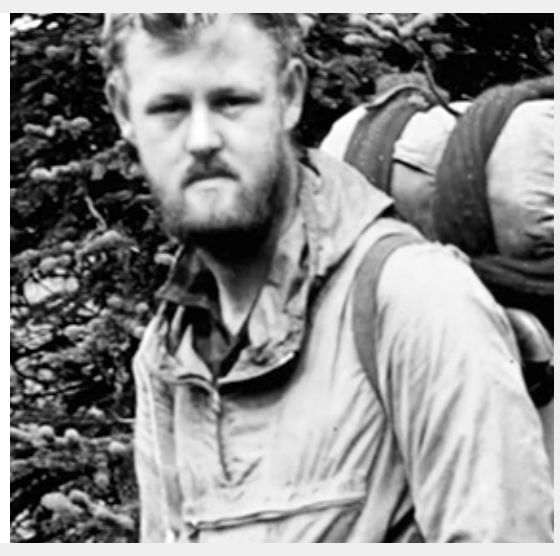
\includegraphics[scale=.3]{images/guy.png}
\caption{Roger Tomlinson inventor of the first GIS system}
\label{fig:guy}
\end{subfigure}
\end{figure}

Geographic Information Retrieval history begins in the late 1940's just after the end of World War II when the United States military began indexing war-time scientific research documents. Although, histories first attempt at mechanized literature retrieval came just before World War I. The first person to build such a system was Emanuel Goldberg \cite{Sanderson:2012cga}. His system successfully searched German microfilm for a pattern of dots. A query that contained a dot pattern would be placed into the machine and a set of microfilm documents would be placed in a film carriage and the machine would systematically search though the documents for the matching set of query dots \ref{fig:first}. This, along with Alan Turing's Theory of Computing and the invention of the transistor, has brought us to our modern state of information retrieval. Another important invention in the history of GIR is the Global Positioning System. The global positioning system is a set of satellites in geostationary orbit that send out a very precisely tuned radio timing signal. When a GPS receiver is receiving at least four of these satellite signals, it can perform a multilateration. Trilateration or multilateration (if more than three satellites) is a mathematical relationship that creates a system of equations that when solved can produce an individuals exact location on Earth. The GPS project was launched by the U.S. Department of Defense in 1973 for use by the United States military and became fully operational in 1995 \cite{Walker:2007hr}. Roger Tomlinson’s pioneering work to create the Canada Geographic Information System resulted in the first computerized GIS in the world in 1963. The Canadian government had commissioned Tomlinson to create a manageable inventory of its natural resources. He envisioned using computers to merge natural resource data from all provinces. Tomlinson created the design for an automated computing system to store and process large amounts of data, which enabled Canada to begin its national land-use management program. He also gave GIS and GIR its name \cite{Jones:2008isa}.    

\begin{figure}[h]
\centering
\begin{subfigure}[b]{0.4\textwidth}
\centering
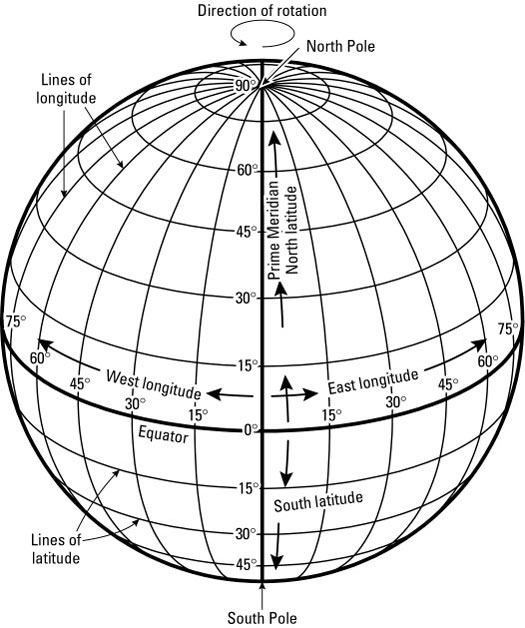
\includegraphics[scale=.3]{images/gps.jpg}
\caption{A geospatial coordinate pair consists of a Latitude and Longitude}
\label{fig:gps}
\end{subfigure}
\begin{subfigure}[b]{0.4\textwidth}
\centering
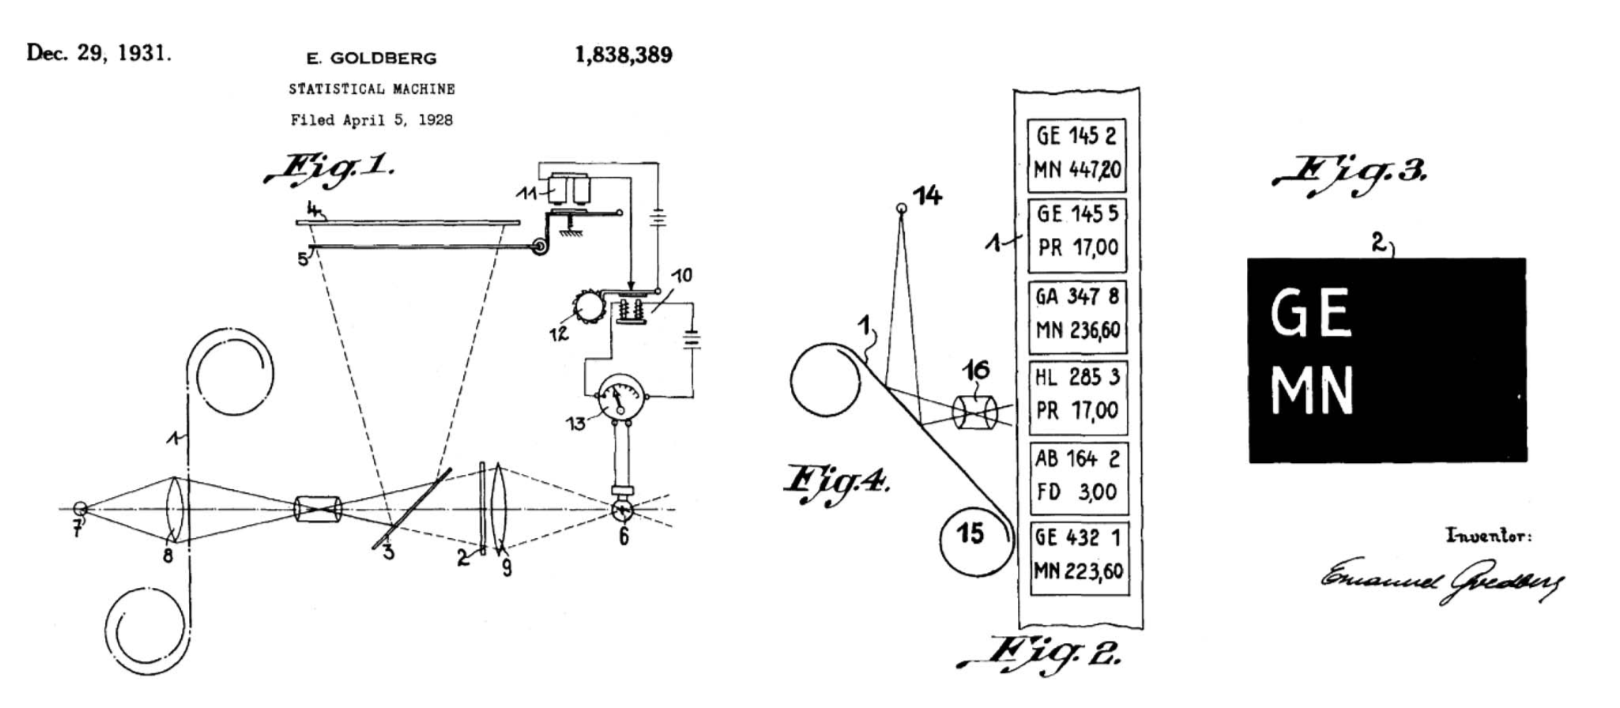
\includegraphics[scale=.2]{images/first.png}
\caption{First device capable of automatic information retrieval}
\label{fig:first}
\end{subfigure}
\end{figure}

 Geographic Information Retrieval is built on the concepts of Information Retrieval. This section covers the basics of the information retrieval model used by modern search engines. The main elements of a IR system consist of
\par
 \begin{itemize}
     \item Information need 
     \item Information resources 
     \item Algorithm for the efficient retrieval of relevant sources 
 \end{itemize}

\textit{Information need} is typically expressed in the form of queries. A \textit{query}: is a request for data usually expressed as a string of unstructured text \cite{Korfhage:2008fe}. \textit{Information resources} typically take the form of unstructured – text, images, video, audio, etc. a web-cralwer would be used to locate these resources \cite{Korfhage:2008fe}. A \textit{Retrieval Algorithm} used to retrieve sources for a given expressed information need is typically executed on a large collection of information sources \cite{Korfhage:2008fe}.
\begin{itemize}
    \item A simple formalization of this algorithm would resemble a tuple \(<f_d,f_q,r>\) where:
    \begin{itemize}
        \item \(f_d\) is a function that maps resources to their representations for retrieval, i.e., \(f_d(d) = x_d\), where \(x_d\) is the retrieval representation of the resource \(d\);
        \item \(f_q\) is a function that maps queries to their representations for retrieval, i.e., \(f_q(q) = x_q\), where \(x_q\) is the retrieval representation of the query \(q\);
        \item \(relevance\) \(r\) is a ranking function
        \begin{itemize}
            \item Takes into account document representation \(xd\) and query representation \(xq\)
            \item Associates a real number that indicates the potential relevance of the document \(d\) for the query \(q\) based on \(x_d\) and \(x_q\);
            \item an example of this \(r\) ranking function could be Google's Page Rank algorithm.
        \end{itemize} and \[relevance(d, q) = r(f_d(d), f_q(q)) = r(x_d,x_q)\]
    \end{itemize}
\end{itemize}


 Information Retrieval is finding information resources usually in the form of documents. These can be of an unstructured nature, usually text relevant to an information need \cite{Korfhage:2008fe}. Geographic Information Systems (GIS) are systems that use theories, methods, technology, programs, and data for learning more about geographic relationships and patterns \cite{Jones:2008isa}. Geographic Information Retrieval (GIR) in the combination of these two fields into a new field of study known as GIR. Thus GIR is essentially a set of techniques for building applications and databases that can index, query, retrieve and browse GEOrefrenced data. The filed of study of GIR is thus trying to better understand and learn from the geographic data that is contained in web documents and user queries. 
 
 \subsection{Main concepts of GIR}
 The main concepts of GIR are very similar to that of traditional information retrieval. Documents can be provided to a GIS system in numerous ways. Traditional GIS would focus on extracting data from large log files such as shipping container histories or population census data \cite{Jones:2008isa}, but more recently the study of GIR has shifted to devising ways to extrapolate geographic data from typical text queries \cite{Long:2018ta}. This type of query is a contrast to the more typical approach to GIS, where specific GEOreferenced data are retrieved from structured databases and the queries are structured in a way that contracts precise GEOspatial constraints such as inputs into address fields \cite{Larson:1996wq}. Documents are also obtained in more traditional methods such as web-crawling. The normal process of extracting information from unstructured documents, representing it with appropriate descriptors, and organizing it into structured indexes is no different than traditional IR. In GIR one typically separates text indexing and analysis from the geographic indexing. This two prong approach is illustrated in fig \ref{fig:gir} .
 
\begin{figure}[h]
\centering

\begin{subfigure}[b]{0.4\textwidth}
\centering
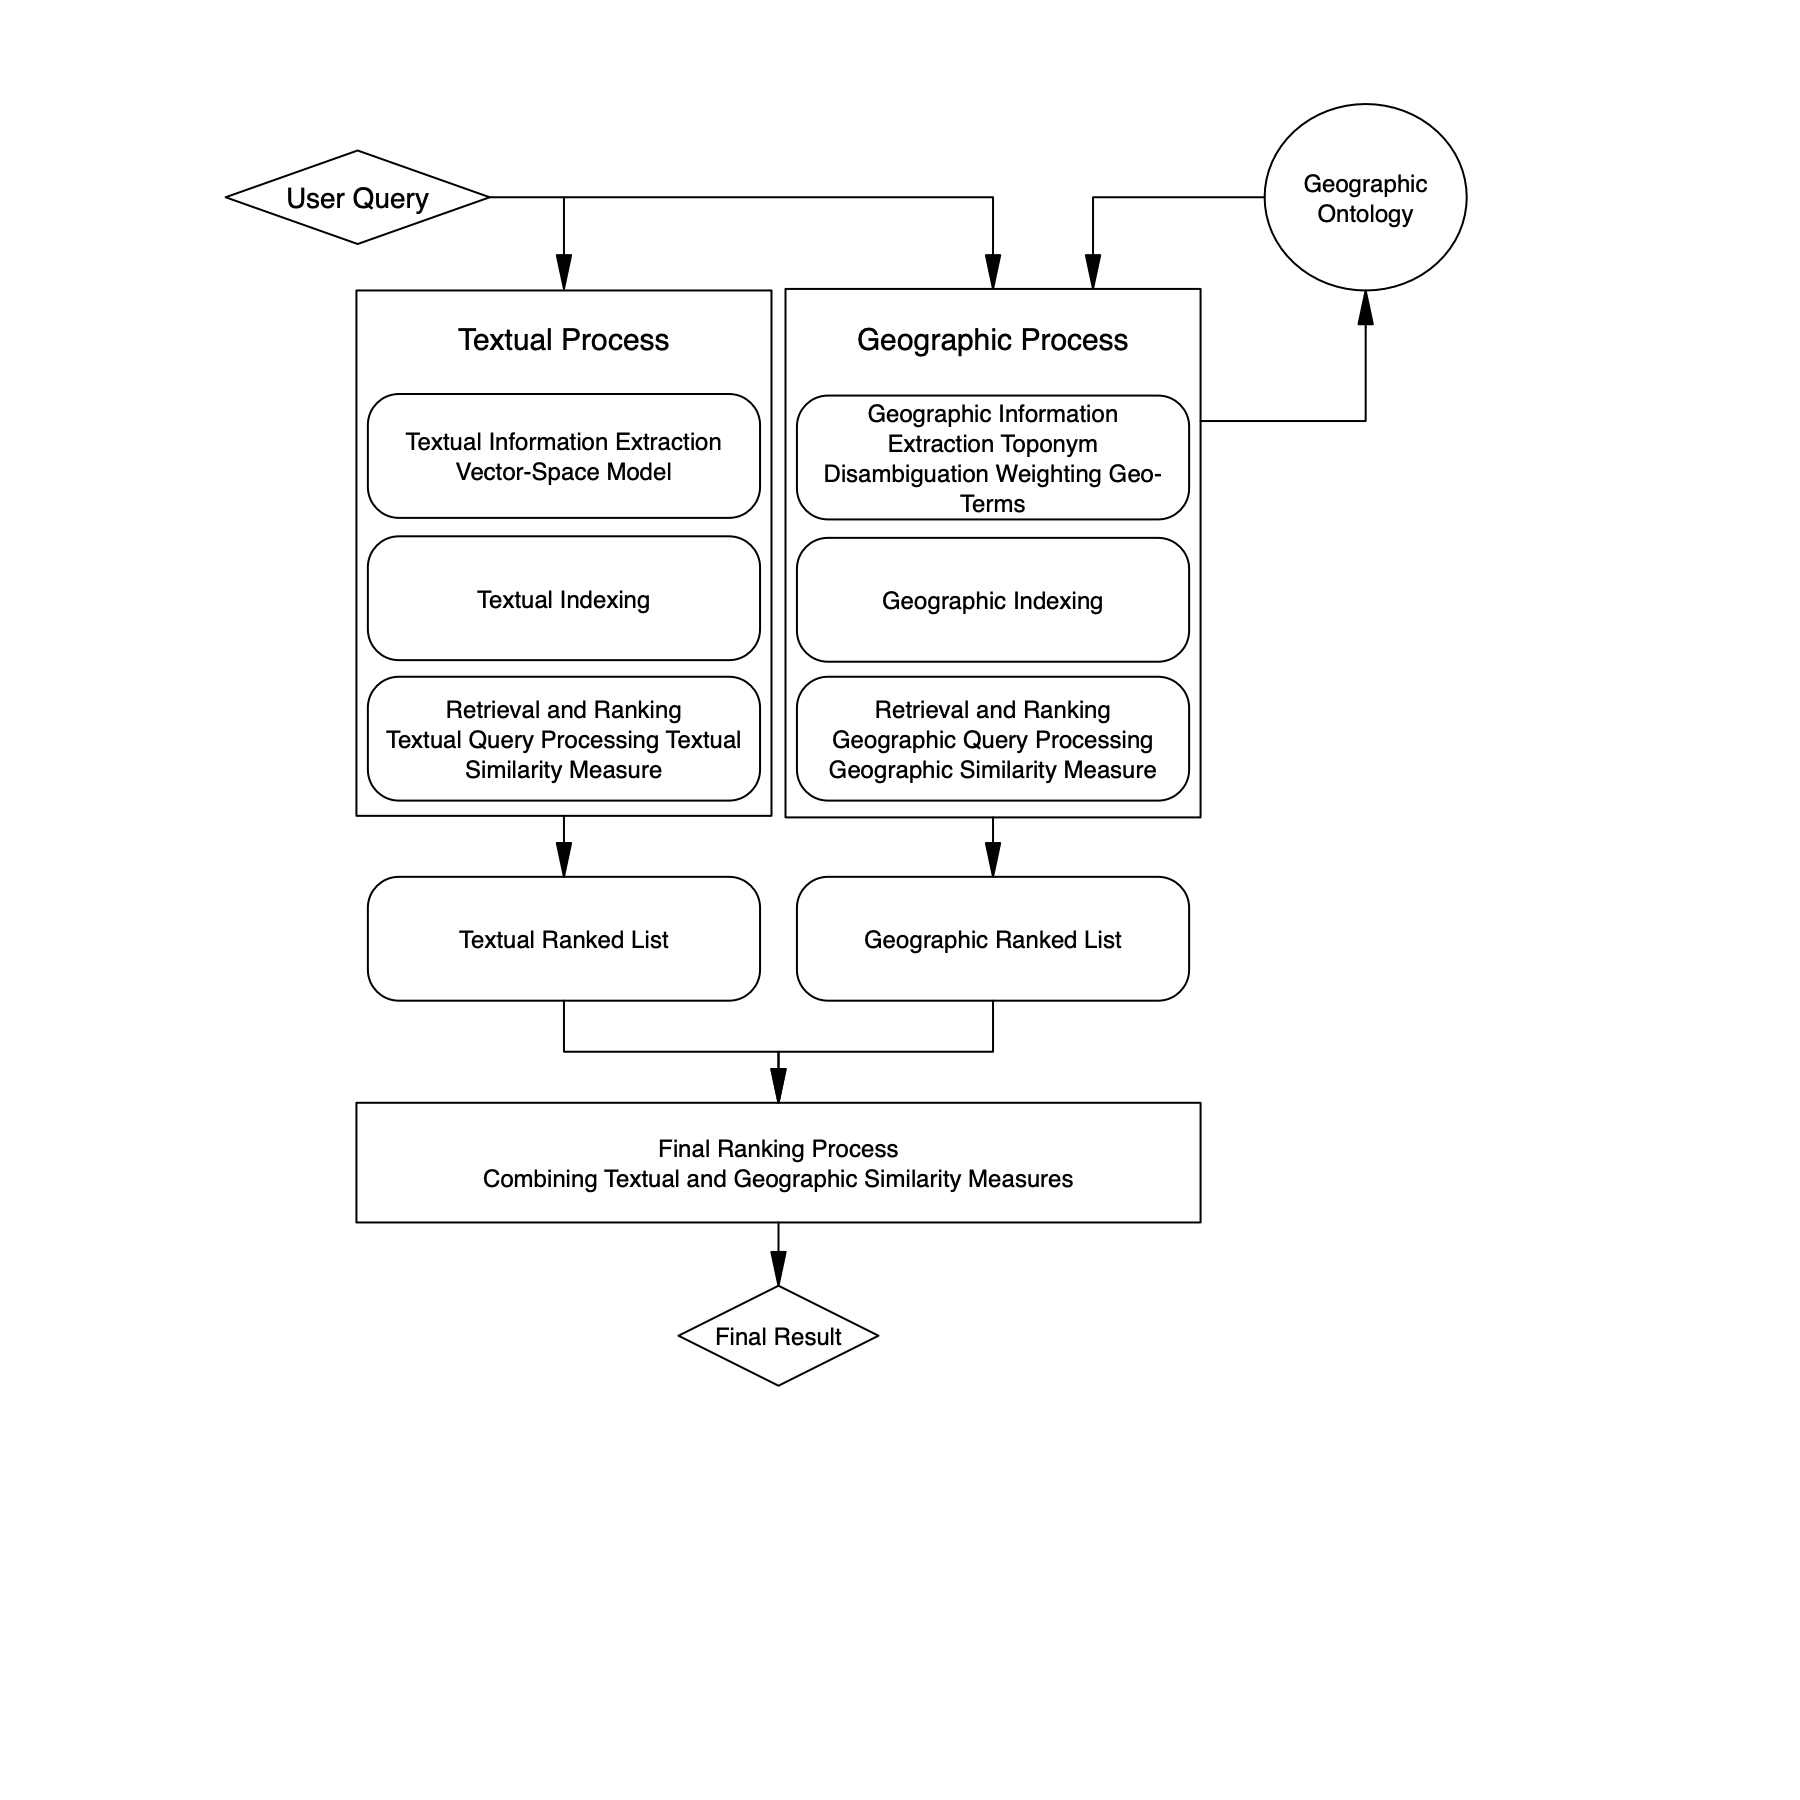
\includegraphics[scale=.2]{images/gir.png}
\caption{A typical GIR process of returning results by obtaining separate results for a text process and geo-referenced process and combining the results}
\label{fig:gir}
\end{subfigure}

\begin{subfigure}[b]{0.4\textwidth}
\centering
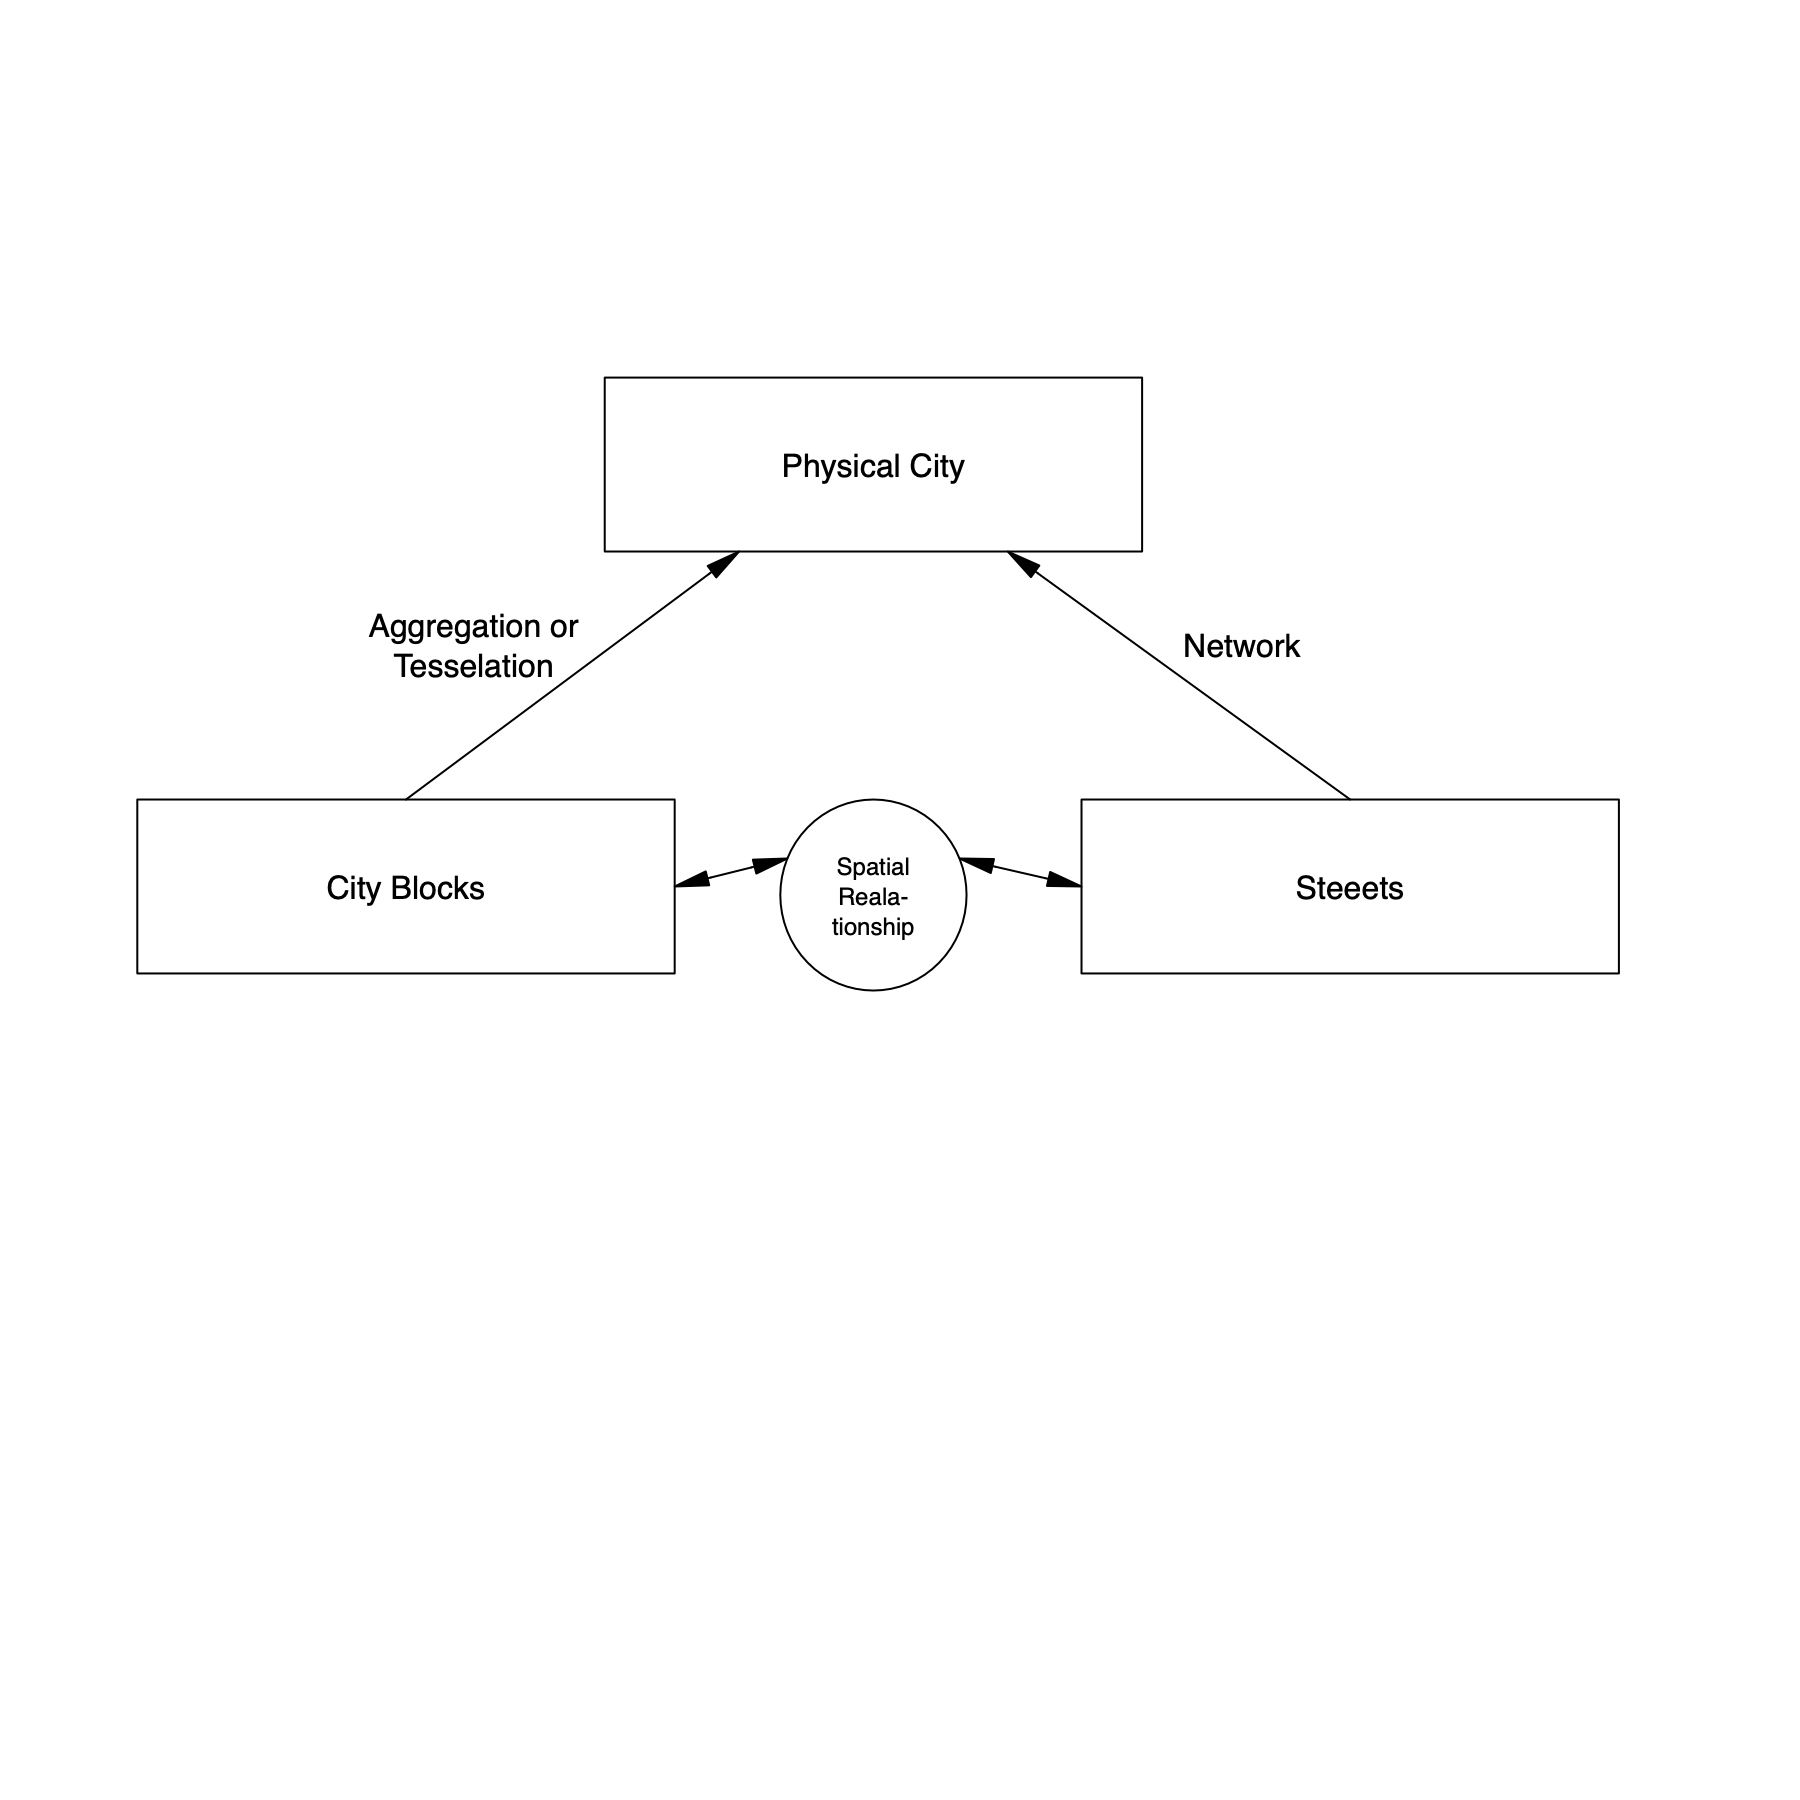
\includegraphics[scale=.2]{images/onto2.png}
\caption{Ontology}
\label{fig:onto2}
\end{subfigure}

\end{figure}

\begin{figure}[h]
\centering
 
\begin{subfigure}[b]{0.4\textwidth}
\centering
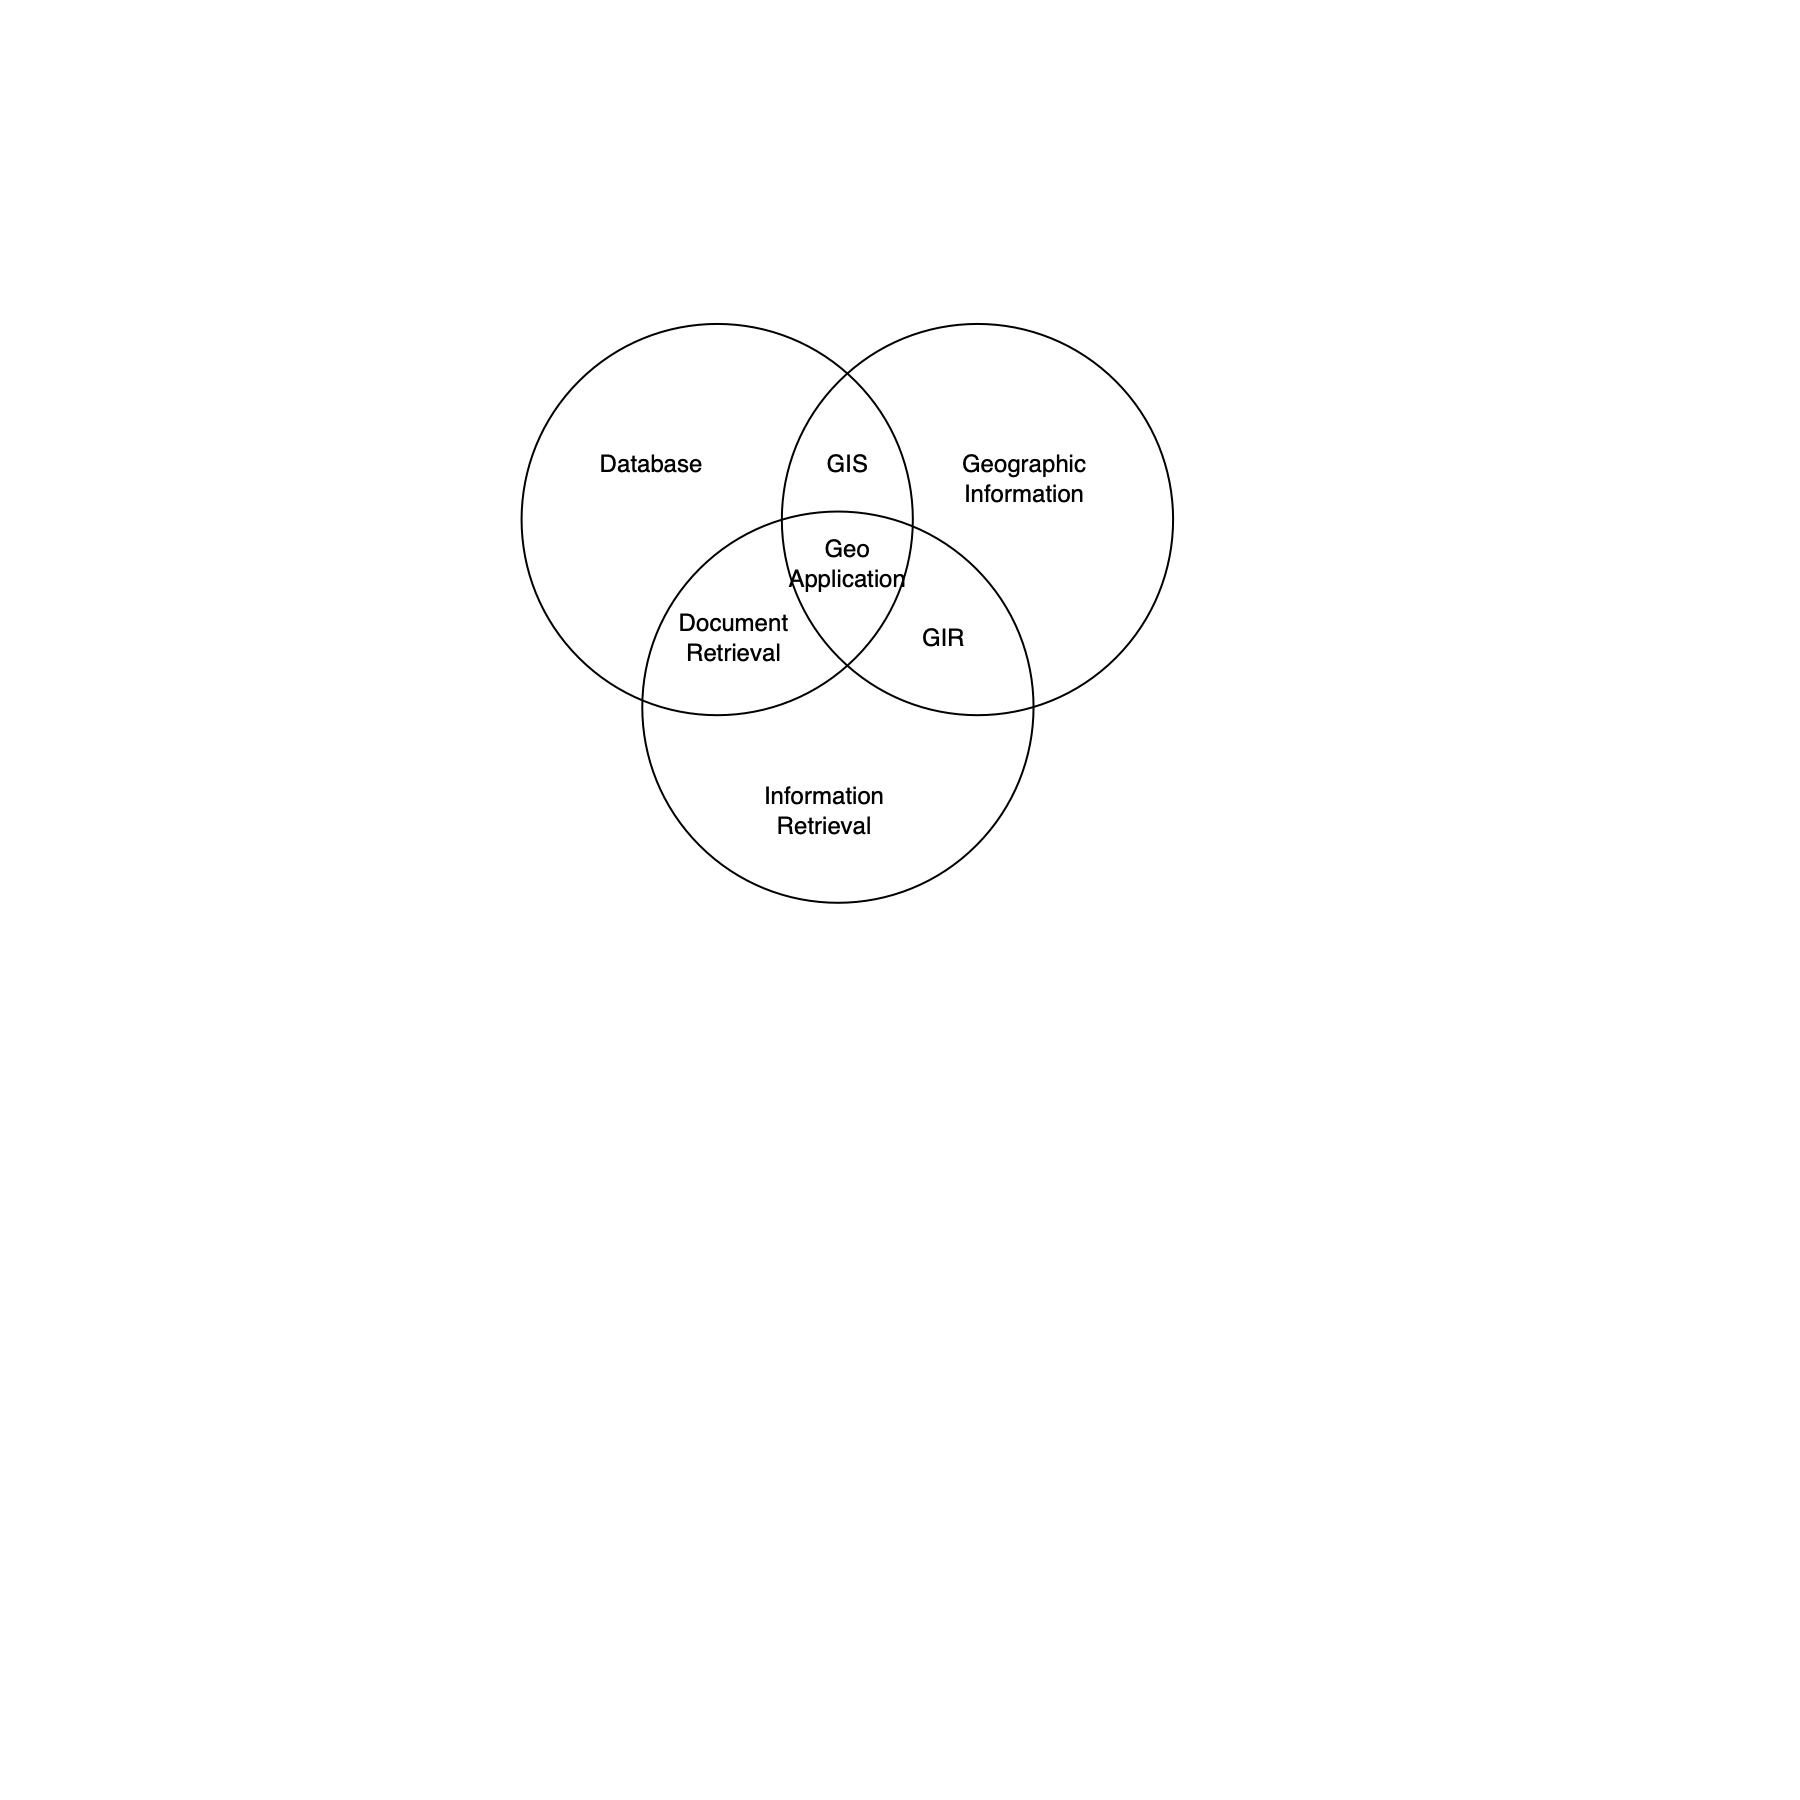
\includegraphics[scale=.2]{images/overlap.png}
\caption{Venn diagram of how GIS, GIR, and IR space's relate}
\label{fig:overlap}
\end{subfigure}

\caption{Flow Visualization}
\begin{subfigure}[b]{0.4\textwidth}
\centering
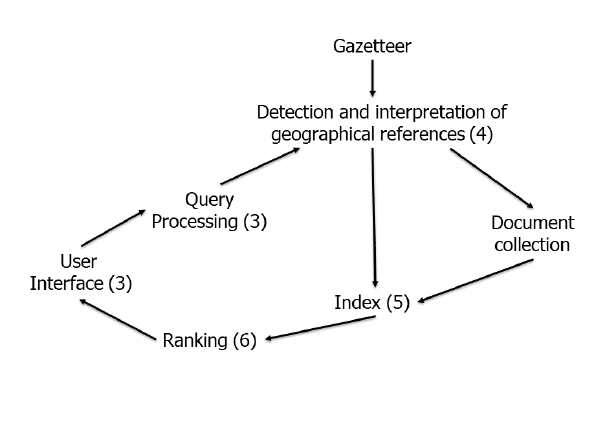
\includegraphics[scale=.5]{images/onto.png}
\caption{Schematic conceptual diagram of a GIR system}
\label{fig:onto}
\end{subfigure}

\end{figure}
 
\subsection{General architecture}
The basic GIR architecture is depicted in figure \ref{fig:gir}. There are multiple ways to return GIR results. The typical architecture that most are familiar with is a text based search that returns a list of places that are geographically near to the search query. Such as searching for Starbucks and being returned a list of the closest Starbucks to your location. The other main types of GIR architecture is entering a text address and being returned a map showing a set of turn by turn directions from our current location to the location that most closely matched the input text. These two examples illustrate the main two architecture types used in GIR. The first general architecture is first creating a ranked list of results using natural language processing techniques. A rank result list is returned by the textual process, and this returned list is then run through the geographical process. Here the results of our textual process are translated to points on a map by the geographical process. In the other version of this, the query is first run through the geographical process, and then the textual process. This is analogous to someone searching for the nearest restaurant. The geographic process returns all restaurants within its interpretation of near, and then the textual process orders the results returned by the geographic process, possibly based on reviews or other criteria. 
\section{Geographic Indexes}
\subsection{Separate Index}
\subsection{Hybrid Index}
\subsection{Use of R-tree structure}
\section{GIR resources}
\subsection{Gazetteers}
A geographical gazetteer is a alphabetical list of places. Each place has some associated information. A geographical gazetteer can be used to locate places with similar names. A geographical gazetteer is made up of three or four main components. 
\begin{itemize}
    \item Alphabetical List
    \item Dictionary
    \item Encyclopedic
    \item A shape file if the location is not a single point i.e. all of London
\end{itemize}
A geographical gazetteer's alphabetical list places names and locations as well as multiple names for the same location in a sort of geographical thesaurus. The dictionary is where the geographical coordinates are typically stored as well as descriptions of its spatial relationships, meaning if its a city, what state does it belong to, etc. The Encyclopedic is similar to both the alphabetical list and the dictionary, but the encyclopedic has more detailed information that may come in the form of articles or long form descriptions. The last type of information that is looked up in a geographical gazetteer is the shape file. The shape file is a file containing a series of points or some form of polygon that defines the shape of the geographic area in question. This shape file is really made up of two distinct types of data. There are shape files that contain raster data and there are shape files that contain vector data. The name Shape file is deceiving because the file is made up of at least four parts. The .SHP, the .DBF, the .PRJ, and the .SHX. 
\begin{itemize}
    \item{SHP: This file contains the geometry of each feature.}
    \item{DBF: This is a database file which contains the attribute data for all of the features in the dataset.}
    \item{SHX: The .shx is the spatial index, it allows GIS systems to find features within the .SHP file more quickly.}
    \item{PRJ: The .prj is the projection file. It contains information about the “projection” and “coordinate system” the data uses.}
\end{itemize}
Each shape file must contain only one geometry. This means that for every geometry required in the data set point, line, or polygon, a separate shape file is required. Another file type for storing geographic information in databases or gazetteers is geoJSON. GeoJSON is JSON or, to give it its full name, JavaScript Object Notation, which is a lightweight data interchange format. It’s primarily used by software developers due to the ease with which it can be processed by web applications. GeoJSON is a form of JSON that also contains geometry data \cite{Butler:2016ev}. Lastly, there is KML. This is the format most likely to be known by non-GIS users, as it is the default file format of Google Earth and is not really used outside of Google Earth and Google Maps \cite{Long:2018ta}. Popular examples of geographic gazetteer's are Getty Thesaurus, GEOnet Names, and Place Name Sites \cite{Ding:1910wl}.  

\begin{figure}[h]
\centering
\begin{subfigure}[b]{0.4\textwidth}
\centering
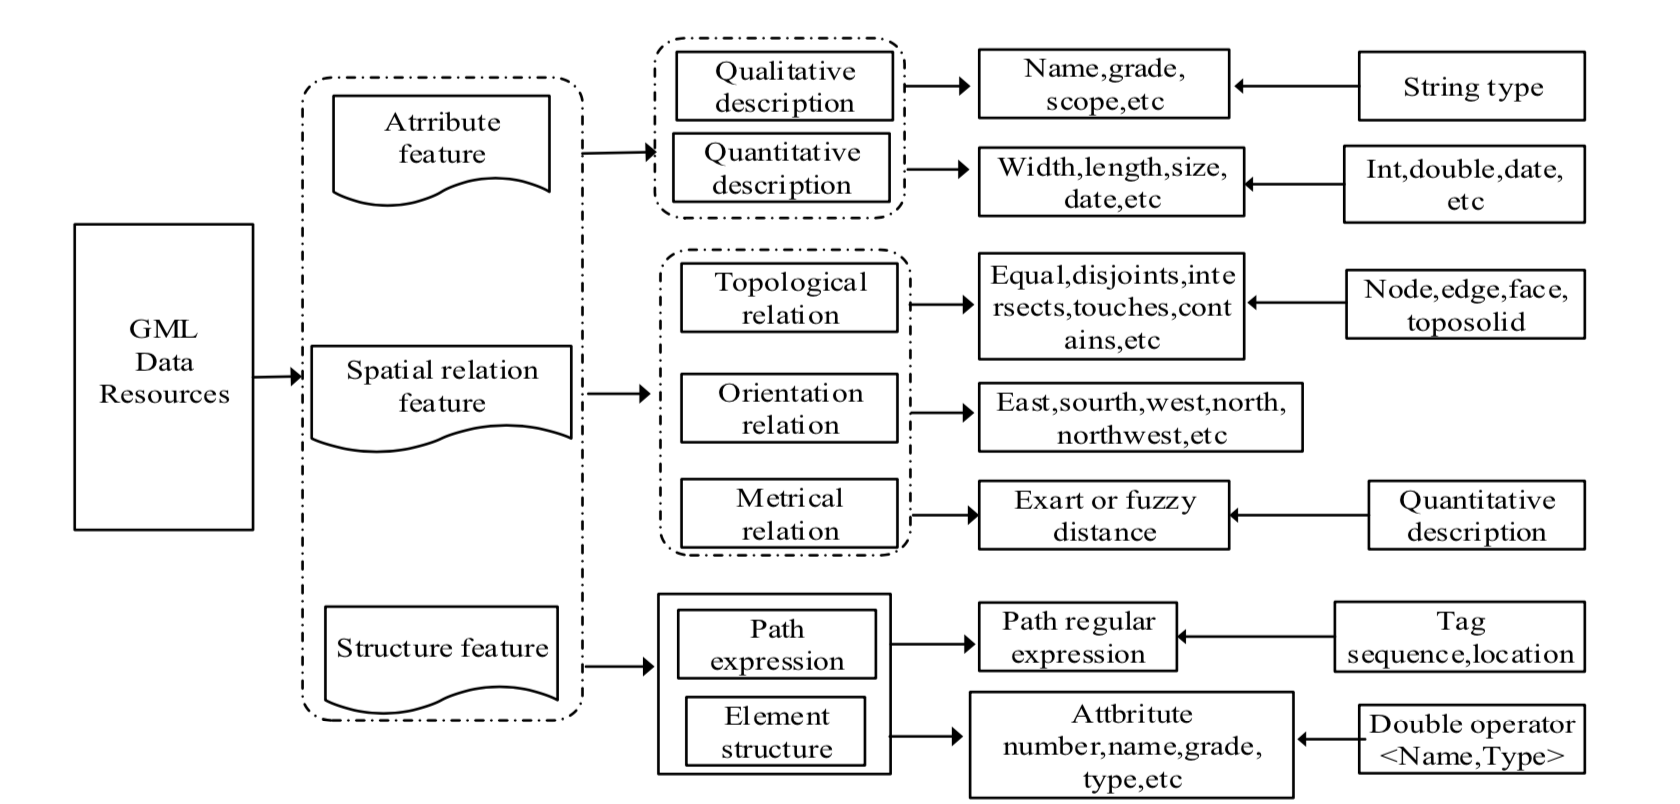
\includegraphics[scale=.2]{images/example.png}
\caption{Example of the type of data stored in a Geographic Markup Language or geoJSON document}
\label{fig:example}

\end{subfigure}
\begin{subfigure}[b]{0.4\textwidth}
\centering
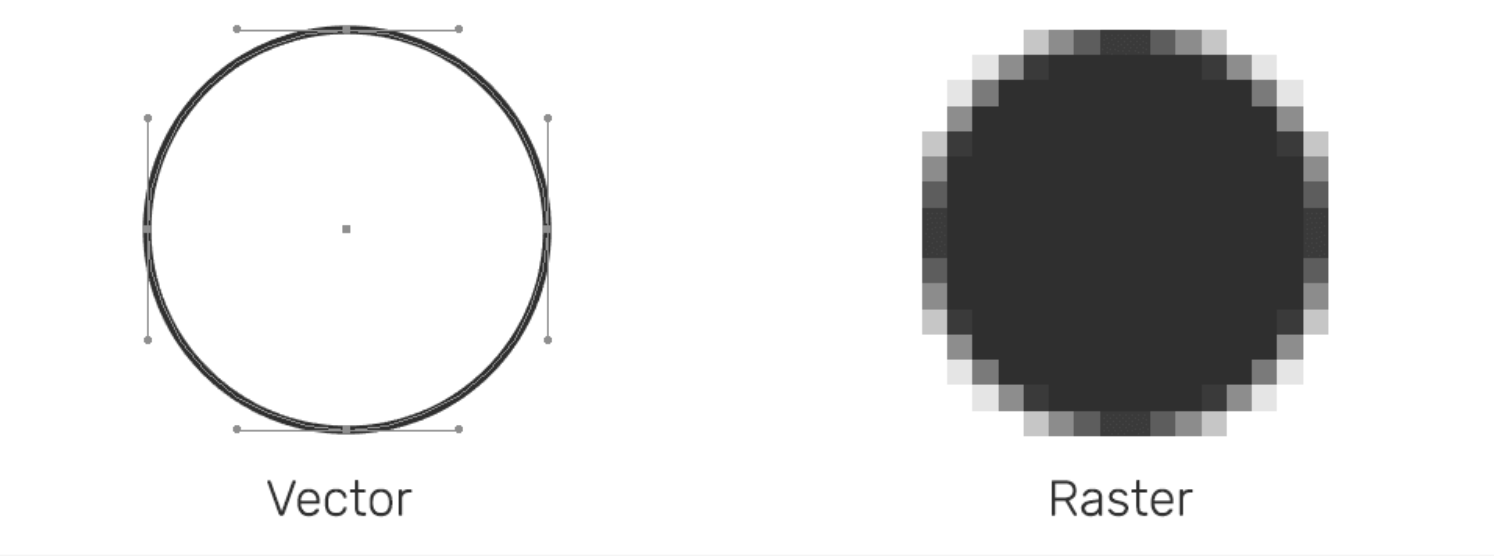
\includegraphics[scale=.2]{images/vec.png}
\caption{Example of the difference between vector and raster data}
\label{fig:vec}
\end{subfigure}
\end{figure}

\subsection{Geographic Ontologies}
A general ontology is a combination of the representation, formal naming, and definition of the categories, properties, and relations between the concepts, data, and entities that substantiate one, many, or all domains \cite{Buttcher:2016vr}. Thus a geographic ontology is specifically any entity that can be assigned a location on the surface of the earth. Semantic relations among these entities can include hyponymy and synonymy relations. Spatial relations among these entities can include near, far, North, and South. The development of geoontologies is important to allow the sharing of geographic data among different communities of users \cite{Fang:2018jc}. It is usually the first communities that spring up on the web that get to decide the format or schema for their types of data; it is no different for geoontologies. The foremost players in geoontologies are 
\begin{itemize}
    \item Yahoo! GeoPlanet: Over 6 million named places, uses web services to unambiguously geotag data across the web. Uses a hierarchical model to build in natural geographical relationships
    \item GeoWordNet: GeoWordNet is a combination service of WordNet and GeoNames. It has 3.5 million named geographical entities.
    \item  GeoNames: Is an OpenSource project with over 10 million geographical names. The Geographical data includes names of places in various languages, elevations, population and others, from various sources. It is the Wikipedia of atluses. Users are allowed to enter and edit entries themselves.
\end{itemize}
\section{Geographic Information Extraction}
One of the main focuses of GIR research is in geographic information extraction. Geographic information extraction is the process assigning a geographic location to every known document on the web \cite{Purves:2018ke}. This is the domain of geographic geotagging webcrawlers. Using techniques developed by research in natural language processing, documents are parsed for certain geographical terms that are used to determine the geographical scope of a document. These commonly looked for terms are:
\begin{itemize}
    \item Place names: Seattle, Mnt. Rainer, Italy, etc.
    \item Geographical relationships: North, South, near, far, within 5 miles, etc.
    \item Geographical concepts: lakes, rivers, towns, cities, etc.
    \item Geographical adjectives: Irish, Eastern, Western, etc.
    \item Geographical coordinates: pairs of Latitude and Longitude, -122.34, 34.34, etc.
    \item Geographically identifying data: Ip addresses, zip codes, street address
\end{itemize}
Geographical scope is the intended range or size of the polygon that the site or document is most related to. An example would be a local hardware store's information page with its address and hours. This could be referenced to a specific point on a map, where as a site about fishing at Mount Rainer has no specific address or point on a map, but is clearly scoped to the mountain itself. Different website intend to reach different geographical regions. For this reason, a website's geographical scope is determined so that a search engine's search results can be tailored to show results that are locally relevant to the user. This process of geographical information extraction is called Geographic indexing. Geographic indexing is typically broken into a two step process, the first being GEOparsing and the second GEOtagging \cite{Larson:1996wq}. GEOparsing is the process of taking a free unstructured text query and transforming it in to an unambiguous geographical identifier \cite{Jones:2008isa}. The most common of these geographic identifiers would be a coordinate pair, typically latitude and longitude. A subset of GEOparsing is GEOcoding, which places more required structure on the input. GEOcoding is typically used to standardize addresses when a user's inputs are incomplete or they enter an ambiguous address. A proper standardized address is then returned \cite{Purves:2018ke}. 
\subsection{GeoTagging}
GEOtagging is the process of attaching geospatial meta-data to documents such as photos. The first step in GEOparsing, as in any query, is Natural Language Processing. Natural Language Processing (NPL) is a large part of IR research and as such a large part of GIR. NPL is a sub-field of IR that studies in particular how to program computers to understand and process human language. GIR researchers need to use natural language processors that contain a component that recognizes geospatial terms. LongPipe and OpenNPL are natural language processors that contain spatial named entity recognition \cite{Page:2015fya}. These natural language processors detect geographical references in the form of places and spatial natural language qualifiers such a near or far. GIR researchers use NLP to help in the interpretation of ambiguous place names such as ball field or nearest grocery store as well as dis-ambiguous place names such as Starbucks \cite{Mountain:2007gc}. 
\subsection{Toponym Recognition}
Place names, or toponyms as GIR researchers like to say, tend to be named after people such as Washington. This makes tokenizing and properly identifying place names and spatial quantifiers particularly difficult. The process of analyzing text is used to identify the presence of toponyms and other spatial quantifiers, determining the genuine geographical occurrences of place names rather than when they are being used to refer to non-geographical terms. Once the text query is properly tokenized into toponyms and spatial quantifiers, the process of matching these tokens with real world places and maps begins. To solve the problem of matching tokenized place names with real-world places that have coordinates and spatial relationships, a geographical gazetteer is used. Once the geographical gazetteer has done its best at matching the unambiguous toponyms, it returns a set of coordinates or list of ranked coordinates ranked on closest possible match to search query. 
\subsection{Toponym Disambiguation Techniques}
There are many techniques to determine a document's scope. Disambiguation toponyms are the main problem that must be overcome when determining a document's scope. Techniques such as Woodruff and Plaunt compute the geographic scope of a document based on the references that appear in the text. This method is based on disambiguating the geographic references using gazetteers to find the shape file. The geographic scope of the document is computed using the overlapping area for all the shape files and trying to find the one place that is related to all the places found in the text \cite{Woodruff:1993wh} A. G. Woodruff, GIPSY: Georeferenced Information Processing System. In \cite{Ding:1910wl} J. Ding, L. Gravano, and N. Shivakumar, “Computing Geographical Scopes of Web Resources,” In Proceedings of the International Conference on Very Large Data Bases, vol. 45, pp. 1–12, Jan. 2010. is a technique also based on the geographical scope like Woodruff and Plaunt, but Ding introduces the idea of Power and Spread to decide the geographical scope the creator of web page intends to reach. Ding proposed two kinds of resources for the calculation of a web page’s geographical scope: the locations of the pages linking to web resource \(ω\) and the place names appearing in \(ω\). \cite{:2005dm} B. M. 0001 and M. J. Silva, “A Graph-Ranking Algorithm for Geo-Referencing Documents.,” ICDM, pp. 741–744, 2005. First, all relevant terms are extracted from the documents and categorized into the correct ontology. This method used the GeoNames public geo-ontology. Now, each document is tagged with its own terms that were found and matched in the geo-ontology. Depending on the frequency of the occurrence of the term, each is assigned a corresponding weight. A weighted graph is used to represent the association between the geographical references and the ontology concepts. Each geographical concept present in the document is assigned a node and a two-way directed edge joins related concepts. Different types of relationships are given different edge weights. A PageRank formula based on edge and node weights is used to compute the ranking score for each node in the graph. The placename with the highest weight is finally assigned as the geographical scope of the page \cite{:2005dm}. \cite{Amitay:2004ju} E. Amitay, N. Har'El, R. Sivan, and A. Soffer, “Web-a-where - geotagging web content.,” SIGIR, p. 273, 2004. describes Web-a-wheres method of first creating a large hierarchical gazetteer containing the hierarchical relationships between geographical data. street/city/county/state/USA/North America etc. The technique then uses this hierarchical gazetteer to create a hierarchy of every term found in the document. They assign each term a weighted value by its level in the hierarchy, then sort the nodes by these values and select the most relevant placenames as the geographical focus of the document. The last technique is sadly the one that is most used and a documents location is simply assigned to a geographical scope at the country level. This technique simply uses the document's country of publication as its document scope.
\section{Geographic Data Representation}
As mentioned earlier, a geographic data representation usually comes in the form of a shape file that either describes the entity as a line, polygon, or point. The geographical data can be represented by 
\begin{itemize}
    \item vector data: vector data is instructions for how to render data. Mathematical instructions that describe a polygon, line, or points. Vector data is abstract.
    \item Raster data: Raster data is literal. Raster data is a bitmap image such as a TIFF or PNG. This format is usually used for formats that are captured digital and as such can only be rendered properly at certain scales. Examples would be satellite imagery, aerial photography, elevation models, and topographic maps.
\end{itemize}
\subsection{Geographic coordinates}
All geographic data usually has at least one reference to a Latitude and Longitude pair to locate the remaining points or secondary coordinate system to a location on earth. Latitude specifies the north-south position on a coordinate pair. Parallel lines of constant latitude circle the earth. The lines run east to west as circles parallel to the equator. Latitude is used together with longitude, which is a similar segmenting of the earth surface. This time the lines run from north to south to determine the east–west position of a point on the Earth's surface. It is an angular measurement, usually expressed in degrees minutes seconds each of which is an angular division of the Meridians lines. These lines connect points with the same longitude. By convention, one of these lines is considered the position of 0 degrees or the Prime Meridian as it is known, which passes through the Royal Observatory, Greenwich, England \cite{Larson:1996wq}. Together a latitude and longitude pair precisely locate a position on the surface of the Earth /ref{fig:gps}.
\subsection{Minimum Bounding Rectangle}
The most common vector data is used when possible as its accuracy does not change with changes in scale. This data is stored in a shape file, but what is this shape that the shape file stores? I have talked of lines, polygons, and points, but most commonly the shape file contains a type of polygon known as a Minimum Bounded Rectangle (MBR). A minimum bounded rectangle is a coordinate pair that defines a rectangle by defining two corners and having lines extend directly North, South, East, and West until they cross with the same lines from the other coordinate to form a rectangle. The MBR is very computationally efficient and its minimal storage requirements make it the most commonly used spatial approximation. However, there are disadvantages associated with the MBR. MBR commonly overestimates the area it is approximating, and it cannot represent complex shapes or places that are not represented as a singular place. 
\section{Geographic Similarity Measures}
To paraphrase a famous geographer named Waldo Tobler, while everything is related to everything else, things that are close together tend to be more related than things that are far apart. In traditional Information Retrieval, scores are based on term frequency or other scores based on the content of the text. In GIR, scores a based on a measure of geographic similarity and are returned as ordered list depending on the similarity measures. Examples include size, shape, and distance. The Measure of Geographic similarity is another major area of research in GIR. The methods for geographic similarity came from Archaeology. Assume an archaeologist finds an ancient village and wants to find more villages. Where is the best place to look? Geographically similar areas with the same soil type, distance from water, elevation, steepness of slope, etc. are ideal. The military is also highly interested in geographic similarity. They use this information to look for targets based on maps, imagery, and digital elevation data. These measures can help them determine likely hiding places by finding other places that are geographically similar in steepness of slope, distance from roads, and distance from known lairs. Geographic similarity measures are most commonly used to simply find how close one place is to one another, so a GIR system can return the nearest.

\subsection{Euclidean distance}
The most commonly used Geographic similarity measure is Euclidean Distance. In terms of GIR, Euclidean Distance is the measure of the proximity between document scope and query scope. GIR ranking methods are based on quantifying the similarity between the query and a document in the collection. In the Cartesian coordinate system, if \(p = (p_1, p_2,..., p_n)\) and \(q = (q_1, q_2,..., qn)\) are two points in Cartesian space of n dimensions, then the minimim distance \((d)\) from point \(p\) on the earth to \(q\) on the earth, or from \(q\) to \(p\) is given by the Pythagorean formula:

\begin{gather*}
(\mathbf {p} ,\mathbf {q} )=d(\mathbf {q} ,\mathbf {p})\\
\\
={\sqrt {(q_{1}-p_{1})^{2}+(q_{2}-p_{2})^{2}+\cdots +(q_{n}-p_{n})^{2}}}\\
\\
={\sqrt {\sum _{i=1}^{n}(q_{i}-p_{i})^{2}}}   
\end{gather*}

\subsection{Topological relationship}
GIR ranking methods are based on quantifying the similarity between the query and a document in the collection. The geographic similarity score can be calculated in innumerable ways. Common measures of topological relationships can be found in table \ref(tab:simg) 


\section{Textual and Geographic Rankings}
 For geospatial searches, the query is compared with MBRs of all candidate documents using polygon-polygon geometric operations. If there is any joint area, overlap, or one area contained within another between the query and the document regions, the document is considered a match. The degree to which the query and the document regions match can be used as a ranking system for returned results. if \(g = 1\) geographic similarity is an exact\\ match if \(g = 0 \) then there is no similarity (see table \ref{tab:simg})
\subsection{First textual, after geographic or vice-versa}
\subsection{Linear combination}
\begin{table}[h!]
\centering
\caption{Other Measures of Geographic Similarity}
\label{tab:simg}
\begin{tabular}{|l|l|}
\hline
\multicolumn{2}{|c|}{
\textit{
\textbf{
Hill \cite{Hill:1990vu} \(g=2\cdot\frac{o}{(q/c)}\)
}}} \\ 
\hline
\multicolumn{2}{|c|}{
\textit{
\textbf{
Walker \cite{Walker:2007hr} \(g=min(\frac{o}{q},\frac{o}{c})\)
}}} \\ 
\hline
\rowcolor[HTML]{E1E1E1} 
\multicolumn{1}{|c|}{\cellcolor[HTML]{E1E1E1}\textbf{Variable}} & \multicolumn{1}{c|}{\cellcolor[HTML]{E1E1E1}\textbf{Denotes}} \\ 
\hline
\textit{q} & area of query region \\ 
\hline
\textit{c} & area of candidit document region \\ 
\hline
\textit{o} & area of overlap between \(q\) and \(c\)\\ 
\hline
\textit{g} & geographic similarity: 1 = match 0 = no similairity \\ 
\hline
\end{tabular}

\end{table}
The other possibility for determining geographic similarity is to use the text of the search itself.  
The similarity measurement of textual geographic information turns to the semantic similarity between two place names. When geospatial propositions are too complex, qualitative methods cannot be used and arbitrary geospatial propositions are used instead \cite{Larson:1996wq}. Then the propositions should be converted into geospatial coordinates, and the spatial similarity is calculated based on quantitative methods, such as overlapping area or Euclidean distance \cite{Jones:2008isa}. 
\section{GIR evaluation}
Information retrieval has long suffered from having no way to truly quantify from one person to the next how relevant the results are. As with typical Information retrieval searches, the information need and the ability of the returned results to match that information need is subjective. In the case of GIR, there is still a lot of subjectivity about returned results; however, a basis for comparison is a lot easier in GIR when the query is the closet restaurant and the algorithm really does return the nearest restaurant. Then there is really no subjectivity. This means that GIR research focuses on the non-subjective measures of evaluation of returned results. Evaluation forums are the accepted method of evaluating IR systems. These forums typically use the Crainfeild method. GeoCLEF is the Geographic track at the CLEF (Cross Language Evaluation Forum) forum for comparing IR systems augmented with geographic data. It is the standard for evaluating GIR systems. The crainfield methdology involves a standard tuple of a corpus, queries and relevance judgments \(<C, Q, R>\) The corpus \(C\) is a collection of documents, the queries \(Q\) a set of requests for information, and the relevance judgments \(R\) a set of documents from the collection that fulfill each information request. 
\section{Conclusions}
With the ever expanding territory of the internet and the Internet of Things, Geographic information systems and geographic information retrieval systems will become more and more indispensable. With our ever expanding population, increasing frequency in natural disasters, and the threat of pollution, Geographic information becomes more important than ever. Everything from fire fighters having the ability to take photographs while around the edge of a wild fire in order for data to be aggregated to create a distinct outline of the fire in real time, to being able to walk into a super market and pick any item up off the shelf and just walk out and be charged automatically are possible with the foundations of the GIS and GIR systems we are building today. Like all new technologies, uses we have yet to even think of will be driving change in tomorrows society. 

\bibliographystyle{IEEEtran}
\bibliography{main.bib}



% that's all folks
\end{document}


